\section{Leveraging Practitoners Feedback to Improve Precision}
\label{sec:intro}

Software configuration management and deployment tools like
Puppet\footnote{\url{https://puppet.com/}}, 
Ansible\footnote{\url{https://www.ansible.com/}},
and Chef\footnote{\url{https://www.chef.io/}} became 
popular amongst software development warehouses~\cite{8919181,rahman2017factors}. 
The adoption of these tools has increased with the growing 
movement to run software in cloud servers. These tools help 
infrastructure teams increase productivity by automating various 
configuration tasks (\myeg{}, server setup). 
In short, these tools describe the environment configuration in 
a set of provisioning scripts that can be versioned and 
reused. They enable configuration consistency between different 
environments and can reduce the time required to provision and 
scale the infrastructure.
The process of managing and provisioning infrastructure through 
configuration scripts is called Infrastructure-as-Code (\iac). 
\iac\ tools take a script as input and create an infrastructure 
that typically runs in a virtual environment as output.

%
As with any piece of code, IaC scripts are also prone to defects 
such as security vulnerabilities~\cite{8812041}. For example, 
in $2020$, Palo Alto Network researchers reported the discovery 
of over $199$K vulnerable IaC templates~\cite{paloalto-unit42}. 
Specifically, $42\%$ of AWS CloudFormation templates, $22\%$ of 
Terraform templates, and $9\%$ of Google Kubernetes YAML files 
were vulnerable. In addition, researchers found more than $67$k 
\textit{potential} security smells in \iac\ scripts implemented 
in Ansible, Chef, and Puppet~\cite{9388795} through an ad-hoc 
tool created to show the presence of a new set of anti-patterns 
for security in the \iac{} domain. 
These reports highlight the importance of tools to prevent 
vulnerabilities from reaching production and shift security left 
in the development pipeline. 

%
Figure~\ref{lst:manifest-example} shows an example of an
\textit{Admin by default} weakness (CWE-250\footnote{CWE-250 details
available at \url{https://cwe.mitre.org/data/definitions/250.html}}),
a potential vulnerability in a Puppet manifest in a module of the
\texttt{PuppetLabs}.\footnote{Admin by default example available at 
\url{https://github.com/puppetlabs/puppet\_operational\_dashboards/blob/9eb67a407aa44c2f924f67f207edc7032f81f86a/manifests/profile/dashboards.pp\#L137} (Accessed \today)}
The vulnerability manifests when the developer
configures a user as ``admin'' or ``root'' for an
infrastructure component. In this example, the \texttt{\$grafana\_user}
is set as ``admin'' for the different services (Puppetserver, Puppetdb, Postgresql, Filesync) used by Grafana\footnote{Grafana is an open-source software
application for data exploration and visualization.
More information available at \url{https://grafana.com/}}. Therefore, 
any service can be prone to a privilege escalation attack.
In \iac{}, all the infrastructure components
are configured through scripts, including the access credentials.
Specifying default users as administrative gives privileges to users
that only an administrator should have. Admin accounts can be exploited 
to access sensitive data and execute unauthorized
code/commands. Infrastructure engineers should avoid setting admin
passwords and usernames to user accounts that do not need the privileges.
Detecting these issues automatically essential to 
make infrastructure engineers aware of possible security problems and
to help companies build more robust infrastructures.


\begin{figure}[t!]
  \centering
  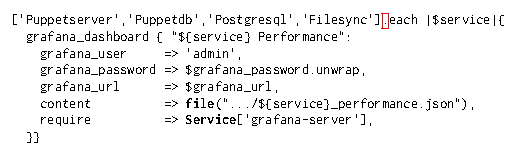
\includegraphics[width=\linewidth]{Figures/Figure-1.pdf}
  \caption{Simplified example of an \textit{Admin by default}.}\label{lst:manifest-example}
  \vspace{-3ex}
\end{figure}


\vspace{1ex}\noindent\textbf{Problem: Puppet IaC Security Linters are not reliable yet!}~In $2019$, Rahman~\etal{}
showed that \iac\ scripts---just like any piece of code---are not immune to security
vulnerabilities~\cite{8812041,10.1145/3408897}. They focused on Puppet configuration files and listed seven
anti-patterns that could lead to security vulnerabilities. The work led to the development of \slic,
a linter to detect those defects in Puppet scripts. Linters are often
imprecise tools~\cite{6606613,7781843,10.1145/1646353.1646374,8622456,8530713,46576}.
Therefore, motivated by the report of very high accuracy (i.e., precision and recall)
from their paper (Table IV~\cite{8812041}), we
decided to conduct a reproduction study of \slic{} based on a
different and larger set of projects. We asked students (co-authors of
this paper) and developers to analyze the warnings that the tool reports.
To validate the students observations of low precision, we reported a sample of the
warnings of the tool to maintainers of \botTotalRepos\ open-source projects. From
the \botTotalIssues\ issues created, we obtained responses to
\botTotalIssuesAnswers\ issues where only \botFinalIssues\ issues were discussed or clear. 
Results showed that the tool performs differently in a new 
set of projects, particularly when validated by the software owners. 
The precision observed was 
smaller than the one reported in SLIC's original 
paper (\botPrecision\ instead of $99\%$)
which indicates that security IaC linters for Puppet
are not reliable yet due to the high false positive rates.

Like many linters, \slic\ uses simple rules to detect issues.
Essentially, it searches for string patterns in
the values of tokens (many times) regardless of their 
type (e.g., variable, string, etc.)
and the relationship between them. For instance, the
``Usage of Crypto. Algorithms'' checker  
(CWE-326\footnote{CWE-326 details are available at \url{https://cwe.mitre.org/data/definitions/326.html}})
searches for any token whose value includes \texttt{sha1} or \texttt{md5}.
Both are built-in Puppet functions and \slic{} fails to consider
the context of usage of these algorithms, i.e.,
these functions are called in Puppet manifests to
encrypt data (e.g., \CodeIn{$encrypt\_key = md5($key)}).
Therefore, \slic{} incorrectly detects 
\CodeIn{md5checksum = '07bd73571b7028b73fc8ed19bc85226d'} as a CWE-326. 
This simplicity creates much noise for developers. In this preliminary study, 
we observed that the rules for the current IaC security anti-patterns 
must be better designed to be safely adopted by the industry and avoid 
productivity disruption.

\vspace{1ex}\noindent\textbf{Solution:}~Our preliminary study revealed
that (1) there is a need to improve the precision of IaC security linters for Puppet, 
and that (2) security tools can be iteratively improved and extended by incorporating 
feedback from the developer community as suggested in previous work~\cite{46576}. 
This paper reports on 
the process we followed to iteratively and 
incrementally improve the precision of an IaC linter according to user 
feedback. For example, the experiments described above ignited 
discussions with members of the development and security teams of 
Puppetlabs\footnote{GitHub PuppetLabs
organization website: \url{https://github.com/puppetlabs}}, as well as one
project manager from Vox Pupuli\footnote{Vox Pupuli is the organization responsible for maintaining
modules and tools for the Puppet community: \url{https://voxpupuli.org/}}.
The feedback collected from the team, OSS maintainers and the Puppet 
community led to the creation of a new tool, which we dubbed as \toolname{}.
Later, we leveraged the expertise of practitioners experienced 
in IaC tools or security to iteratively and incrementally
improve the new tool.

Figure~\ref{fig:timeline} shows the timeline of feedback collection 
followed to design and improve \toolname{}.
To sum up, we bootstrapped the design of \toolname\ with rules obtained 
from the revision of SLIC's ruleset, according to the feedback of the 
research team and owners of OSS projects (\textit{phase 1} in
Figure~\ref{fig:timeline}); and, incrementally evolved the linter
according to the recommendations of practitioners
(\textit{phase 2} in Figure~\ref{fig:timeline}). We improved
\noRulesSlic\ rules of the \slic{} ruleset and added
\newRules\ new rules that were either recommended by practitioners (e.g. weak
password); or relevant for the infrastructure domain (e.g. homograph
attacks\footnote{Apple Domain Attack (2017):
\url{https://www.xudongz.com/blog/2017/idn-phishing/}} and malicious dependencies).

\begin{figure}[t!]
  \centering
  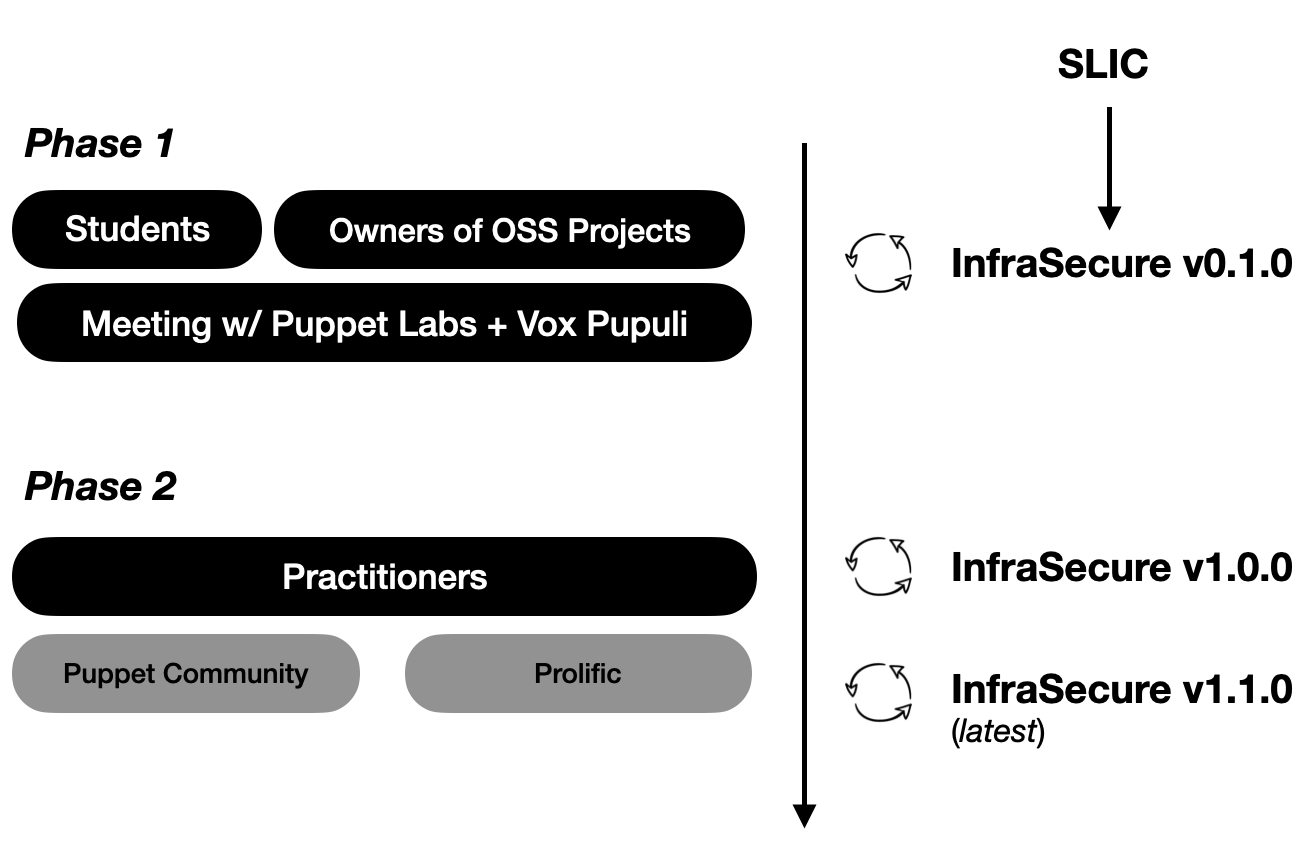
\includegraphics[width=\linewidth]{timeline.png}
  \caption{Timeline of feedback collection.}\label{fig:timeline}
  \vspace{-3ex}
\end{figure}

\vspace{1ex}\noindent\textbf{Main Results:}
This paper performs the following contributions:

\begin{itemize}[topsep=.2ex,itemsep=.2ex,leftmargin=0.8em]
    \item[\Contrib{}]\textbf{Study.}~A replication study of \texttt{SLIC}'s precision,
    including a preliminary study conducted with two researchers (co-authors of this paper)
    and a study with several \github\ scripts validated by project maintainers;
    \item[\Contrib{}]\textbf{InfraSecure.}~A new linter
    adjusting \noRulesSlic\ rules of the original
    \slic\ ruleset and adding \newRules\ new rules with a final precision of \finalPrecision.
    \item[\Contrib{}]\textbf{Dataset.}~A dataset of \iac{} scripts with more than $1000$ warnings
    classified as false positives and true positives that researchers can use to evaluate
    other security linters;
\end{itemize}

\noindent\textbf{\textit{Take-away message:}}~The takeaway message of
this paper is that it is feasible to tune security linters to produce
acceptable precision for important classes of warnings (confirming the
findings reported in a study at Google~\cite{46576}) and
that involving practitioners in discussions is an effective way to
guide the improvement of those linters.

\noindent\textbf{\textit{Replication Package:}}~All the scripts and data
    used in this study (including feedback obtained from the maintainers and practitioners)
    are available at: \repPackage{}.

	%%%%%%%%%%%%%%%%%%%%%%%%%%%%%%%%%%%%%%%%%%%%%%%%%
\section{Background}\label{sec:background}
%%%%%%%%%%%%%%%%%%%%%%%%%%%%%%%%%%%%%%%%%%%%%%%%%

This section provides background information on Puppet and
discusses security weaknesses in \iac\ scripts.

\begin{table}[!t]
  \small
  \centering
  \setlength{\tabcolsep}{3pt}
  \caption{Examples of security smells per weakness.}
  \vspace{-2ex}  
  \label{tab:examples}
  \begin{tabular}{ll}
   \toprule
   \textbf{CWE}   &  \textbf{Example} \\\midrule
   CWE-798  & \$username = ``mariadb''\\
   CWE-259  & \$password = ``!TQ23Rg''\\
   CWE-321  & \$key = ``A67ANBD7''\\
   CWE-319  & \$req = ``http://www.domain.org/secret'' \\
   CWE-546  & \#https://bugs.debian.org/cgi-bin/bugreport.cgi?bug=538392 \\
   CWE-326  & password => md5(\$debian\_password) \\
   CWE-284  & \$bind\_host = ``0.0.0.0'' \\
   CWE-258  & \$rabbitmq\_pwd = ``'' \\
   CWE-250  & \$user = ``admin'' \\
   CWE-521  & pwd => ``12345'' \\
   CWE-1007 & \$source = "http://deb.debi\mhl{a}n.org/debi\mhl{a}n" \\
   CWE-829  & \$postgresql\_version = 8.4 \\
   \bottomrule
  \end{tabular}
  \vspace{-2ex}
\end{table}

% %
\subsection{Puppet}

Developers no longer
deal with systems composed of a single machine and database.
Instead, system administrators must manage multiple diverse operating systems, databases, and virtual machines.
Perhaps most importantly, they must ensure their
configurations are consistent at any given time. Configuration management
technologies have been around for over a decade---Puppet was founded in $2005$.
Puppet is a solution that helps IT infrastructure management through 
code by supporting software deployment, packages,
and configuration. In Puppet, programs
are written using Puppet's declarative language. They are
called manifests. More information about the language can be found 
elsewhere\footnote{More about Puppet: https://puppet.com/docs/puppet/7/puppet\_overview.html}.


\subsection{Security Weaknesses}

This section describes in more detail the potential weaknesses 
in Puppet scripts. Table~\ref{tab:examples} illustrates 
examples of each weakness.

\textbf{Hard-coded secrets (CWE-798):} This warning refers to the practice of
including sensitive information such as passwords or cryptographic keys in
code files. Table~\ref{tab:examples} shows a hard-coded 
password example.
Rahman \etal{} considered $3$ kinds of data as
sensitive: usernames, passwords, and cryptographic keys. 
However,
the Common Weakness Enumeration\footnote{CWE-798 description is available at \url{https://cwe.mitre.org/data/definitions/798.html}}
list does not consider solo hard-coded usernames as a threat.
Practitioners
involved in our validation studies shared the same opinion. Therefore,
we argue that hard-coded usernames should be only reported
when there is a paired password (CWE-259) or cryptographic key (CWE-321).
More discussion on this is provided later in Section~\ref{sec:design}.


\textbf{Use of HTTP without TLS (CWE-319):} This warning refers to the practice
of using HTTP without the Transport Layer Security (TLS) to transmit
sensitive data. This means that attackers can more efficiently exploit the
communication channel as the data is transmitted unencrypted, as
cleartext\footnote{This type of issues can lead to man in the middle (MITM) attacks: \url{https://owasp.org/www-community/attacks/Man-in-the-middle_attack}}.

\textbf{Suspicious comment (CWE-546):} This warning refers to
 comments that suggest the presence of bugs, missing security functionalities,
or weaknesses of a system. Details provided in comments about bugs, security functionalities
or weaknesses can be crucial for hackers to exploit the infrastructure.

\textbf{Use of weak cryptography algorithms (CWE-326):} This warning refers to
using weak crypto algorithms.
Attackers can easily crack the encryption schemes and have
access to the data~\cite{10.1007/11426639_2}.

\textbf{Invalid IP address binding (CWE-284):} This warning refers to
assigning the address 0.0.0.0 to a server.
This practice allows connections from any IP address to access 
that server~\cite{DBLP:conf/raid/Mutaf99}.
While mail servers have to listen on 0.0.0.0 to receive
mail, database servers should not since it can lead
to critical data breaches.

\textbf{Empty password (CWE-258):} This warning refers to using
empty strings as passwords, which are easily
guessable.

\textbf{Admin by default (CWE-250):} As detailed in the Introduction, this warning refers to
defining users with administrative privileges. This can result in security
weaknesses since it can disable or bypass security checks performed by the system.\footnote{Why
you should not use an admin account: \url{https://www.lbmc.com/blog/why-you-should-not-use-an-admin-account/}}

\textbf{Weak Password (CWE-521):}
This warning refers to the usage of weak passwords. Weak passwords
are easily guessable and can be bypassed to gain access to systems.

\textbf{Insufficient Visual Distinction of Homoglyphs Presented to User (CWE-1007):}
This warning refers to malicious actors using homoglyphs
that may cause the user to misinterpret a glyph and perform an unintended, insecure action.
The homograph attack performed against the apple website\footnote{Phishing
with Unicode domains:~\url{https://www.xudongz.com/blog/2017/idn-phishing/}} is a well-known
example of this type of weakness. Table~\ref{tab:examples} shows an example of a domain where 
the character ``\mhl{a}'' could be replaced by the respective homoglyph, as in the apple attack.
This warning might be essential to uncover malicious domains implanted by malicious open-source
contributors---typosquatting attacks.\footnote{OpenSSF post on scanning OSS software for malicious behavior:~\url{https://openssf.org/blog/2022/04/28/introducing-package-analysis-scanning-open-source-packages-for-malicious-behavior/}}

\textbf{Malicious Dependencies (CWE-829):} This warning refers to malicious software
by nature, i.e., dependencies that integrate known vulnerabilities (CVEs).
These are the leading cause of supply chain attacks, and one of the main
challenges the security community faces nowadays~\cite{9402108}. 

\section{Preliminary Study}\label{sec:preliminary_study}

This section reports on the findings of two studies---involving
different sets of participants---to assess the performance of SLIC, 
a recently-developed linter for Puppet.


\subsection{Validation with Students}\label{sec:research_team}

This section reports on a study involving two of this paper's 
authors to assess the precision of \slic\ on an
independent benchmark. The study consisted in inspecting
\fpSampleSize{} warnings reported by the tool. The warnings
were validated by one senior PhD student whose research focuses 
on security and static analysis and one junior PhD student 
in software engineering with basic security skills. 

\subsubsection{Dataset}\label{subsec:dataset}

\sloppy
To build our dataset, we mined \github\ projects containing \texttt{Puppet} scripts. 
We used three different queries to search for repositories: 1) \CodeIn{language:puppet is:public}; 2) 
\CodeIn{puppet in:readme is:public}; and, 3) \CodeIn{devops is:public}. We discarded results pointing 
to forked repositories (to avoid duplicates) and discarded results pointing to repositories without 
any code in \texttt{Puppet} scripts. Our crawler found a total of \totalMinedRepos{} GitHub repositories 
and \totalMinedScripts{} associated \texttt{Puppet} scripts. \slic\ scanned these scripts for the
seven sins and reported a total of \textbf{\minedWarnings} security warnings involving 
\minedScriptsWarnings{} \texttt{Puppet} scripts (=$26.5$\% of the total) from \minedReposWarnings{} 
repositories (=$73.5$\% of the total).
Table~\ref{tab:sins_large} shows the breakdown of warnings reported by \slic. Column ``Rule'' shows the name (kind) of the warning, 
column ``\#'' shows the number of warning reports of that kind, and column ``\%'' 
shows the percentage of the total associated with that number. 
This table lists the warnings in order of their prevalence.

  \begin{table}[t]
    \small
    \centering
    \setlength{\tabcolsep}{10pt}
    \caption{\label{tab:sins_large}Breakdown of warnings reported by \slic{}.}
    \vspace{-2ex}
    \begin{tabular}{lrr}
      \toprule
      Rule & \multicolumn{1}{c}{\#} & \multicolumn{1}{c}{\%}  \\
      \midrule
      Hard-coded secrets & \hardcodedSecretsMined{} & 69.9 \\
      Use of HTTP without TLS & \httpWithoutTLSMined{} & 11.7 \\
      Suspicious comments & \suspiciousCommentsMined{} & 8.7 \\
      Use of Weak Crypto. Algos. & \weakCryptoMined{} & 4.7\\
      Invalid IP Address Binding & \emptyPassMined{} & 2.4\\
      Empty Password & \invalidIPMined{} & 2.1\\
      Admin by default & \adminDefaultMined{} & 0.5 \\
      \midrule
      Total & \minedWarnings{} & 100 \\
      \bottomrule 
    \end{tabular}
    \vspace{-2ex}    
  \end{table}


\subsubsection{Methodology}\label{sec:pre_meth} \textbf{Samples.}
Given the high number of warnings reported by the tool (\minedWarnings) and the need for 
humans to analyze each warning, we sampled a set of reported warnings. 
We leveraged two popular complementary sampling strategies to that end~\cite{strat-sampling}. 
\textit{Stratified sampling} is a method to draw samples from a set by taking into account the 
distribution of kinds---in our case, the distribution of kinds of warnings. A \textit{proportional} (stratified) sampler draws samples in a number proportional to 
the size of the sets associated with each kind whereas an \textit{uniform} (stratified) 
sampler draws the same number of samples for each kind.
% To contrast, a proportional sampler 
% draws much more warnings of the kind ``Hard-coded secrets'' compared to ``Admin by default''
% whereas an uniform sampler draws the same number of warnings for both types. 
Intuitively, 
a proportional sampler values more the most prevalent kinds of warnings (as to make more 
accurate measurements on those kinds) whereas an uniform sampler treats every kind equally 
(as to avoid inaccurate measurements on uncommon kinds).
We sampled \proportionalSampleSize{} warnings \textit{proportionally} and \uniformSampleSize{} 
(=36*7) warnings \textit{uniformly}. In total, we analyzed  
\fpSampleSize\ warnings, which is a substantial increase when compared to the 
\akondFpWarnings\ warnings analyzed in the \slic{}'s paper~\cite{10.1145/3408897}. \textbf{Metric.}
We focused on precision to measure the reliability of the reports of 
the tool. 
% Precision is the ratio between the number of true warnings 
% (True positives or TP) reported and the total number of warnings reported by a 
% given tool, including false warnings (false positives or FP). 
% \begin{align}
% 	Precision = \nicefrac{TP}{TP+FP}\label{eq:prec} 
% \end{align}
Precision is especially important for security linters. Reporting scores of false 
warnings can be highly disruptive for a team's productivity, as team members tend 
to interrupt work to address high-priority tasks~\cite{DistefanoEtAlCACM2019}. Developers 
are less willing to use linters with low rates of precision because they find them not 
trustworthy and unreliable~\cite{46576}. \textbf{Statistical Tests.} Each one of the \fpSampleSize\ warnings was 
manually inspected by two co-authors. Cases where the authors found disagreement were discussed to reach 
a consensus. We report on the results of a Cohen's Kappa
analysis~\cite{cohen1960coefficient} to measure the inter-rater 
reliability of human decisions.
%
\subsubsection{Results}

\begin{table}[t]
  \small
  \centering
  \setlength{\tabcolsep}{3.5pt}
  \caption{\label{tab:prel_analysis_slic}Performance of SLIC. (Validation with Students)}
  \vspace{-2ex}
  \begin{tabular}{lrrrrrr} 
    \toprule
    \cellcolor{Gray} \textbf{\slic{}} & \multicolumn{3}{c}{\textit{proportional}} & \multicolumn{3}{c}{\textit{uniform}} \\\midrule
    Rule & \#TP & \#FP & Pr. &  \#TP & \#FP & Pr. \\
    \midrule
    Hard-coded secrets & \tpHardcodedSecretsProportional{} & \fpHardcodedSecretsProportional{} & \precHardcodedSecretsProportional{} & \tpHardcodedSecretsUniform{} & \fpHardcodedSecretsUniform{} & \precHardcodedSecretsUniform{} \\
    Use of HTTP without TLS & \tpHttpWithoutTLSProportional{} & \fpHttpWithoutTLSProportional{} & \precHttpWithoutTLSProportional{} & \tpHttpWithoutTLSUniform{} & \fpHttpWithoutTLSUniform{} & \precHttpWithoutTLSUniform{} \\
    Suspicious comments & \tpSuspiciousCommentsProportional{} & \fpSuspiciousCommentsProportional{} & \precSuspiciousCommentsProportional{} & \tpSuspiciousCommentsUniform{} & \fpSuspiciousCommentsUniform{} & \precSuspiciousCommentsUniform{} \\
    Use of Weak Crypto. Algorithms & \tpWeakCryptoProportional{} & \fpWeakCryptoProportional{} & \precWeakCryptoProportional{} & \tpWeakCryptoUniform{} & \fpWeakCryptoUniform{} & \precWeakCryptoUniform{} \\
    Invalid IP Address Binding & \tpInvalidIPProportional{} & \fpInvalidIPProportional{} & \precInvalidIPProportional{} & \tpInvalidIPUniform{} & \fpInvalidIPUniform{} & \precInvalidIPUniform{} \\
    Empty Password & \tpEmptyPassProportional{} & \fpEmptyPassProportional{} & \precEmptyPassProportional{} & \tpEmptyPassUniform{} & \fpEmptyPassUniform{} & \precEmptyPassUniform{}\\
    Admin by default & \tpAdminDefaultProportional{} & \fpAdminDefaultProportional{} & \precAdminDefaultProportional{} & \tpAdminDefaultUniform{} & \fpAdminDefaultUniform{} & \precAdminDefaultUniform{} \\
    \midrule
    Total & \tpProportionalSample{} & \fpProportionalSample{} & \precTotalProportional{} & \tpUniformSample{} & \fpUniformSample{} & \precTotalUniform{} \\
    \bottomrule 
  \end{tabular}
  \vspace{-5ex}
\end{table}


Table~\ref{tab:prel_analysis_slic} shows \slic{}'s results for both 
sampling strategies:
\textit{proportional} and \textit{uniform}. 
For each sampling strategy, we present the number of true positives~(\#TP), 
the number of false positives~(\#FP), 
and the Precision. Considering the results for \textit{proportional} 
sampling, the authors found a total of \tpProportionalSample{} 
true positives and \fpProportionalSample{} false positives. 
The average precision of \slic\ was \precTotalProportional{} for the 
proportional set. Considering the results for \textit{uniform} sampling, 
the authors found a total of \tpUniformSample{} true 
positives and \fpUniformSample{} false positives. 
On average, \slic's precision was \precTotalUniform{} for the uniform set. 

We ran a Cohen's Kappa analysis to measure the inter-rater reliability of human 
decisions in classifying the warnings. The kappa coefficient ($k$) shows the level 
of agreement between the two co-authors. The analyses yielded $k$=$0.89$ 
and $k$=$0.94$ for the \textit{proportional} and the \textit{uniform} sampling 
sets, respectively. According to McHugh's interpretation of $k$~\cite{mchugh2012interrater}, 
the reported levels of agreement 
are strong and almost perfect for the proportional and uniform sampling sets, respectively. 
For illustration, agreement was reached in $482$ out of $502$ warnings. 
The two co-authors discussed the warnings that 
raised disagreement. Cases where 
consensus was not reached were replaced by a new one and re-evaluated.
Cases where agreement was reached were updated with the final 
conclusion---inferred from the discussion between both co-authors. 

\textit{\textbf{Summary:}} Results show that the original precision of \slic\ drops 
considerably from $99\%$ (reported in the original work~\cite{8812041}) to below $65\%$ 
when tested in a new set of puppet scripts---which might indicate that \slic\ needs to 
be improved. However, the lack of context on the software under analysis by the co-authors 
may also be the reason for a lower precision. Therefore, we conducted a new experiment
with the owners and maintainers of open-source software, i.e., people with more knowledge 
and context of the applications.



\subsection{Validation with Owners of OSS projects}\label{subsec:maintainers}

\sloppy
Complementing the preliminary study reported in the previous section,
this section reports on the findings of a validation study of
\slic\ conducted with the maintainers of open source projects. The
motivation of this study was to confirm the observations of the 
previous experiment but now with open source developers, i.e., 
developers with more context of the software under analysis.  
\github\ issues 
were designed to
illustrate the security smells (including references to the corresponding
CWEs\footnote{Common Weakness Enumeration (CWE) taxonomy available at
\url{http://cwe.mitre.org}.}) and to guide the developer towards
patching the issue. We followed guidelines for issue reporting from
the literature. Issues include code samples, links to more
information and we strive to make the report message as brief and
objective~\cite{carvalho2020c}. Figure~\ref{fig:issue} shows an
example of an issue created for a ``Hard-coded Secret''. The title is
``Potential vulnerability in Puppet file: Hard-coded Secret''. The
issue (1) shows where the potential vulnerability is (code:
\CodeIn{cron\_user = 'root'}, script:
\CodeIn{puppet-apt\_mirror/manifests/init.pp} and line: $191$); (2)
explains the vulnerability and its possible implications (bypass
protection mechanism, gain privileges on applications, and access to
sensitive data); and (3) makes a recommendation to the developer on
how she can fix the vulnerability (by using a vault, in this
case). We created different templates of this message for the
different warning types.

\begin{figure}[t!]
  \centering
  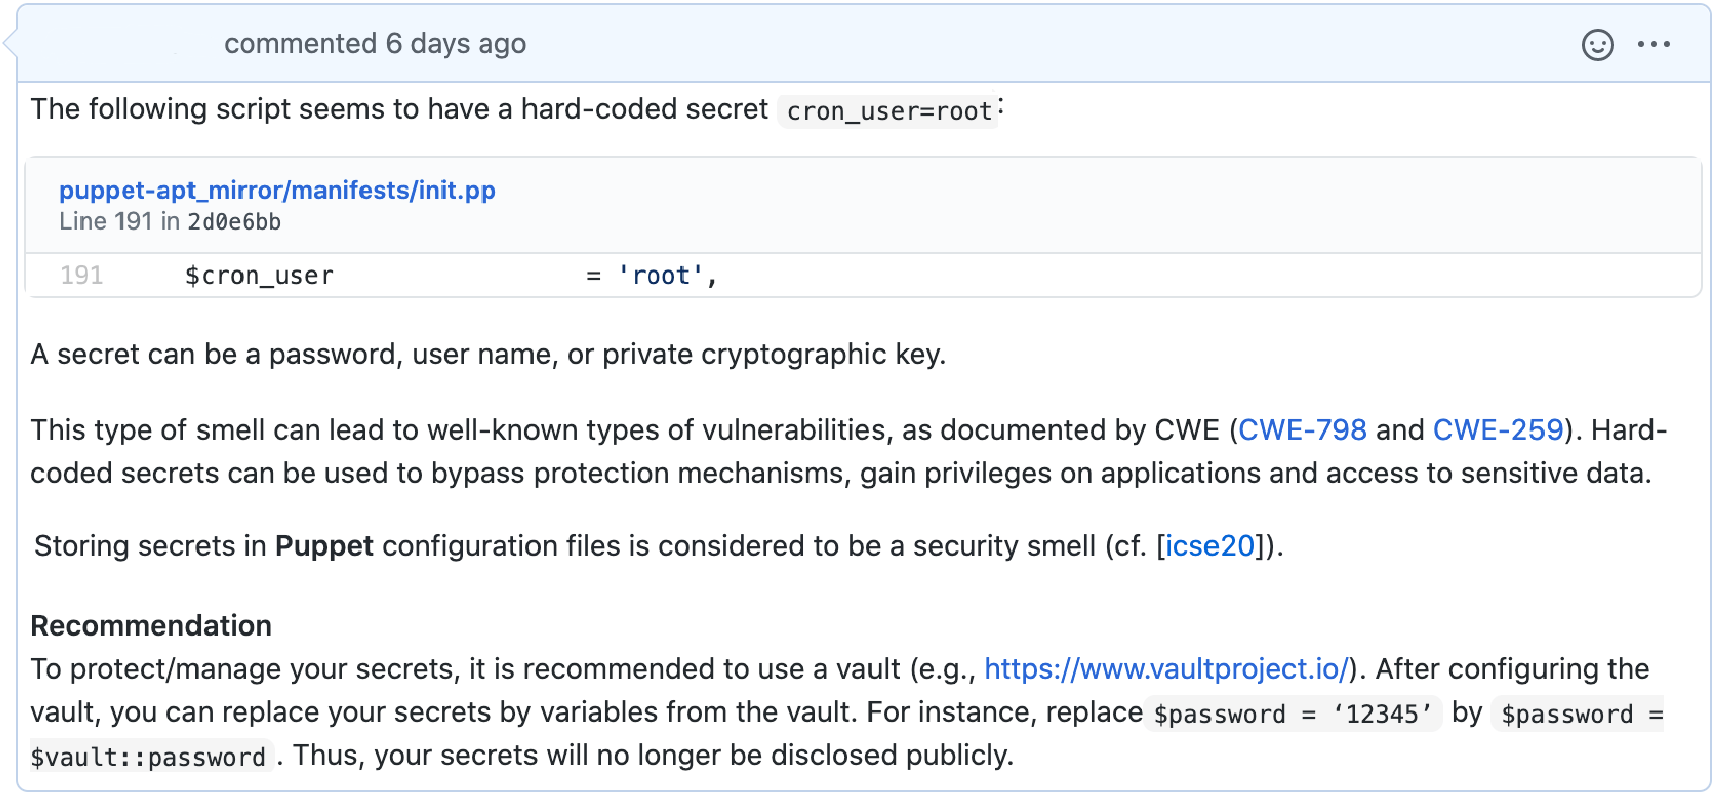
\includegraphics[width=\linewidth]{issue.png}
  \vspace{-4ex}  
  \caption{Example of issue opened (based on SLIC report).}\label{fig:issue}
  \vspace{-3ex}
\end{figure}
%

%
\subsubsection{Dataset}

The dataset used in this study was different from the one from 
Section~\ref{sec:pre_meth}. 
We mined \github\ projects with activity in $2020$ 
(at least one commit) and containing Puppet scripts. 
We conjectured that focusing on projects with recent activity would increase 
our chances of obtaining responses. We used two different queries to search for 
repositories: 1) \CodeIn{language:puppet is:public}; and, 2) \CodeIn{puppet in:readme is:public}. 
We discarded results pointing to forked repositories (to avoid
duplicates), repositories without any activity in $2020$ (no commits),
and repositories without any code in Puppet per project. Our tool
scanned \botTotalScripts{} Puppet scripts from \botWarningsRepos{}
GitHub repositories. In total, \botTotalWarnings{} security warnings
were detected in \botScriptsWarnings{} Puppet scripts (=$30.7\%$ of
the total). We issued alerts to projects with maintainers involved 
in the slack of the Puppet community. We received \botTotalIssuesAnswers{} answers to 
the \botTotalIssues{} issues we submitted, but only \botFinalIssues{}
issues were clearly validated by practitioners---which were 
the ones we considered for our conclusions.

\subsubsection{Methodology} This section presents the methodology 
followed to submit the issues. \textbf{Sample.} A total of
\botWarningsRepos{} \github\ repositories were scanned to this
study. We ensured that the repositories had recent activity (at least
one commit in $2020$) to improve the probability of obtaining
responses. The total amount of scripts scanned was
\botTotalScripts{}
---$7$ times the sample used in our preliminary
study (Section~\ref{subsec:dataset}) and $28$ times the sample used in
Rahman et. al~\cite{8812041} to evaluate the SLIC's precision and
recall. 
\textbf{Issues.} We reached out to the software owners 
through the Puppet community slack and submitted issues to projects 
with maintainers involved in the slack community. All the issues followed
a specific template depending on the type of warning
(cf. Figure~\ref{fig:issue}). The issued message not only located and
explained the vulnerability but also recommended an example of a
patch (i.e., actionable messages to save maintainers time). \textbf{Reply Evaluation.} We monitored the discussion threads
associated with the issues. For each response obtained, we classified
the warnings reported as true positives (TP) or false positives (FP)
according to the opinion of the maintainers in their responses.
Issues closed by the maintainers without any reply or activity were discarded.
Issues closed with unclear responses (e.g., 
``N/A'', ``:thumbs\_down'') were also discarded since they did not provide
clarity on the validation of the issue. We only considered the issues where there was some sort 
of discussion of the issue (e.g., ``These todo's shouldn't be there, I agree ... but it's not about defects/weaknesses here. It's 
just a marker to include more operating systems in the future.'') or a clear validation of the issue (e.g., ``All false positives'', ``This is not a secret.'').
From the answers
obtained, two of the co-authors manually inferred the classification
of each warning. We use Cohen's Kappa~\cite{cohen1960coefficient} to
measure the inter-rater reliability of human
decisions. \textbf{Metrics.} We measured Precision as
described in Section~\ref{sec:pre_meth}. 


\begin{table}[t!]
  \small
  \centering
   \setlength{\tabcolsep}{9pt}
  \caption{\label{tab:maintainers}Performance of \slic. (Validation with Owners\Space{ of OSS projects})}
  \vspace{-2ex}
  \begin{tabular}{lrrr} 
    \toprule
    Rule & \#TP & \#FP  & Precision\\
    \midrule
    Hard-coded secrets & $77$ & $119$ & $0.39$ \\
    Use of HTTP without TLS & $1$ & $72$ & $0.01$\\
    Suspicious comments & $3$ & $15$ & $0.17$\\
    Use of Weak Crypto. Algos. & $0$ & $3$ & $0.00$\\
    Invalid IP Address Binding & $0$ & $1$ & $0.00$\\
    Empty Password & $1$ & $5$ & $0.17$ \\
    Admin by default & $1$ & $0$ & $1.00$\\
    \midrule
    Total & 83 & 215 & 0.28\\
    \bottomrule 
  \end{tabular}
  \vspace{-2ex}  
\end{table}

\subsubsection{Results} This section reports results. \textbf{Issues.} We
reported a total of \botTotalWarnings{} warnings in \botTotalIssues{} issues
($9$ warnings per issue, on average). Project owners responded 
to \botTotalIssuesAnswers{} issues of the \botTotalIssues{}
issues we submitted, but only \botFinalIssues{} issues were clearly discussed 
or validated---the equivalent to \botTotalAnswered{} warnings (Table~\ref{tab:maintainers}). One issue for an
``Empty Password'' warning was fixed by one of the maintainers
(82c3cb7\footnote{Fix for ``Empty password'' issue: \url{https://github.com/jtopjian/puppet-sshkeys/commit/82c3cb7e78c16cf6517207779f79ab5b2a71b603} (Accessed \today)});
one tagged the issue with ``waiting for contribution''; another commented asking to perform a pull request. \textbf{Reply
  Evaluation.} We used the following method to determine the warning
classification (\ie{}, false or true positive) from the answers of
project owners. We discarded warnings related to issues closed without
any response or activity and issues that remained open or without any
response by the time of our analysis. After that stage, two of this paper's co-authors reviewed each of the answered
issues. Each warning received two votes. Then, we ran a Cohen's Kappa
analysis to measure the inter-rater reliability of our choices to
assess the confidence in our classification method. The kappa
coefficient ($k$) shows the level of agreement between the two
co-authors. The analysis yielded $k=1.0$, i.e., a total agreement 
between both co-authors. \textbf{Precision.} Table~\ref{tab:maintainers} shows the
number of true positives~(TP) and the number of false positives~(FP) per
type of warning. In total, \slic\ reported $83$ true positives and
$215$ false positives for the $33$ issues considered, which resulted in
an average precision of $0.28$ for \slic{}. Note that the samples used for 
``Use of Weak Crypto. Algorithms'', ``Invalid IP Address Binding'', ``Empty Password'' and 
``Admin by default'' are relatively small, so results might not reflect the entire reality. 


\textit{\textbf{Summary:}} Results indicate that the precision of
\slic{} is even lower when evaluated by maintainers---developers with 
more knowledge and context of the applications---of the software (drops to $28\%$).
These results confirm our initial observations and indicate that 
better security IaC linters for Puppet are needed.

\section{\toolname: Puppet Security Linter}\label{sec:tool}

The observations described in the previous section motivated the 
pursuit of a more precise security linter for Puppet scripts. 
The previous experiments ignited discussions with members 
of the development and security teams of PuppetLabs, as well 
as a project manager from Vox Pupuli. We leveraged the feedback 
obtained from the previous studies and the professional feedback to
design a new security linter for the Puppet
community, which we dubbed as \toolname{}. More precisely, we created 
a new linter as a result of \textit{phase 1} (Figure~\ref{fig:timeline}) 
and incrementally evolved the linter according to the recommendations of professionals 
(Figure~\ref{fig:timeline}, \textit{phase 2}), improving
\noRulesSlic\ rules of the \slic{} ruleset and adding
\newRules\ new rules. 
The following sections report the new architecture (Section~\ref{sec:architecture}), 
design choices (Section~\ref{sec:design}) and security checkers (Section~\ref{sec:rules}) that resulted
from the feedback collection (Figure~\ref{fig:timeline}): 
\begin{itemize}
  \item \textit{Phase 1}: feedback from the \textbf{owners of OSS projects},  
  \textbf{PuppetLabs} and \textbf{Voxpupuli Engineers} (as described in 
  Section~\ref{sec:preliminary_study}) that led to the creation of \toolname{} (v0.1.0);
  \item \textit{Phase 2}: two cycles of feedback from the \textbf{Puppet} and \textbf{Prolific} 
  communities (as described in Section~\ref{sec:evaluation}) that led to two new releases of 
  \toolname{} (v1.0.0 and v1.1.0);
\end{itemize}


\subsection{Linter Architecture}\label{sec:architecture}

One recommendation from the PuppetLabs team (\textit{phase 1}) was to implement 
the set of the rules as plugins to the \puplint{} architecture\footnote{Puppet-lint website: \url{http://puppet-lint.com/}},
through the \puplint\ check API\footnote{Puppet-lint check API: \url{http://puppet-lint.com/developer/api/}}. 
This API facilitates the integration of new checkers in \puplint\. 
In addition, it allows the user to suppress warnings and disable or enable
checkers---which are regarded as important features by the community. All 
security checks were developed as plugins to \puplint\ (Table~\ref{tab:rules}). 
These checks are applied to the Abstract Syntax Tree (AST) of a Puppet manifest which 
is generated by an internal tokenizer\footnote{Puppet-lint tokenizer: \url{http://puppet-lint.com/developer/tokens/}}.
\toolname\ was implemented in \texttt{Ruby} and its \texttt{CLI} is available 
online\footnote{Gem is available at \url{https://rubygems.org/gems/puppet-lint-infrasecure}}.
The codebase of the linter is available 
at \url{https://github.com/TQRG/puppet-lint-infrasecure} and open to future contributions.

\subsection{Design Choices}\label{sec:design}

This section describes the design choices of our analysis, guided by 
the distinct cycles of feedback as described in Section~\ref{sec:preliminary_study} 
and Section~\ref{sec:evaluation}; also, illustrated in Figure~\ref{fig:timeline}.

\textbf{Variable/Attribute Assignments (VASS).} From the preliminary 
analysis performed in Section~\ref{sec:preliminary_study}, we have noticed 
security-related code smells being detected in logical conditions. For instance, 
\CodeIn{if has\_key(\$userdata, ’env’)} shows a logical condition that 
was incorrectly flagged as a hard-coded secret issue. Aiming to 
reduce the number of incorrect predictions, we implemented a rule to search 
for variable and attribute assignments in Puppet manifests---\texttt{isVarAssign(\textit{token})}
and \texttt{isAtrAssign(\textit{token})} (cf. Table~\ref{tab:rules}).

\textbf{Reasoning about the token value (TOKVAL).} Some of the rules did not 
reason about \texttt{token.value}. For hard-coded secrets, 
the linter only checks if the token value is not empty. While manually validating the 
samples used in our studies, we found false positives of hard-coded secrets. For instance, 
\CodeIn{aws\_admin\_username = downcase(\$::operatingsystem)} which does not store 
any actual secret. \slic{} flagged this case as a hard-coded secret because the value assigned 
to the variable \CodeIn{aws\_admin\_username} is not empty. However, the rule needs to 
reason not only about the length of the right-hand side of the variable assignment but also about 
the type of token and value. \toolname\ locates variable and attribute assignments in the AST and considers 
that secrets are usually stored in \CodeIn{:STRING} and \CodeIn{:SSTRING} tokens. In addition, we defined a database
of known credentials (\texttt{isUserDefault(\textit{token.value})})---credentials that are not 
considered secrets by the community\footnote{\url{https://puppet.com/docs/pe/2019.8/what\_gets\_installed\_and\_where.html\#user\_and\_group\_accounts\_installed}}---and,
invalid secrets (\texttt{invalidSecret(\textit{token.value})}) which are 
consider as non-valid values for hard-coded secrets. The linter ignores all the credentials in this database. Feedback from distinct \textbf{owners of OSS Projects} is what
drove us to make this decision is presented below:

\begin{itemize}[topsep=.2ex,itemsep=.2ex,leftmargin=0em]
  \item[] \textbf{[User Default]}: 
  \textit{``The names of these UNIX accounts are not 
  considered to be secret. They are 
  published openly as part of the PE documentation:
  \url{https://puppet.com/docs/pe/2019.8/what\_gets\_installed\_and\_where.html\#user\_and\_group\_accounts\_installed}''}
  \item[] \textbf{[Invalid Secret]}: 
  \textit{``This are default users and default as found in every installed 
  fpm package. there is most of the time a wwwrun or a www-data user 
  depending on the system.''}
\end{itemize}

\textbf{Use of HTTP without TLS is fine sometimes (SAFE).} As \slic{}, \toolname{} also flags 
every single occurrence of \textit{http://}, i.e., it recommends to use TLS by default. For example, the tool
flags \CodeIn{apturl => "http://deb.debian.org/debian"}, even though it refers to a credible 
source. Our definition of credible source is a source that can be trusted. However, 
different companies can have different opinions regarding the credibility of the same source.
That is why this rule is customizable. We observed that this type of issues (CWE-319) are prevalent in Puppet files. 
Applications often use third-party libraries, which are usually configured in Puppet 
files, and the links to their sources are not necessarily unsafe.
Also, depending on the context of an application, the configuration of 
localhost servers as HTTP may not be a problem. If no sensitive data is communicated, 
then there is probably no problem using \CodeIn{http}. \toolname{} has a configuration file 
for safe domains, i.e., domains that are cleared to be use \CodeIn{http}. Thereby, infrastructure teams can 
customize their own configuration files. The feedback provided 
in Section~\ref{sec:evaluation} from two different \textbf{practitioners}, which
supported this decision, is presented bellow:

\begin{itemize}[topsep=.2ex,itemsep=.2ex,leftmargin=0em]
  \item[] \textbf{[Whitelist]}: 
  \textit{``I think it is fine if localhost is used. Otherwise TLS 
  should be mandatory. All the big 
  financial organizations will not use this check because 
  they cannot create internal certs or use 
  letsencrypt.''}
  \item[] \textbf{[Whitelist]}: 
  \textit{``By default, it's unsafe to not use HTTPS. 
  But for internal testing/development it is acceptable 
  to me to not use HTTPS all the time.''}
\end{itemize}


\textbf{Hard-Coded Secret Division in different checkers (SECR).} 
In Section~\ref{sec:preliminary_study},
we observed that the hard-coded secrets checker produces the most significant number
of alerts. For instance, \slic{} assumes a secret is a key, password or username. 
As mentioned previously in Section~\ref{sec:background},
the Common Weakness Enumeration list does not consider solo 
hard-coded usernames as a threat. Practitioners involved in our validation 
studies shared the same opinion. 
We analyzed the distribution of the different types of hard-coded secrets
and realized that $48\%$ of the secrets detected were usernames.
Therefore, in the final version of our tool, we decided
to separate the hard-coded secrets checker into three new checkers (one per type of secret). This 
way, developers can disable the username checker if they find it 
noisy. We did not delete the original checker; infrastructure
teams can use it if they want to collect all the different 
types of secrets simultaneously. Feedback provided 
in Section~\ref{sec:evaluation} from a \textbf{practitioner} 
supported this decision:

\begin{itemize}[topsep=.2ex,itemsep=.2ex,leftmargin=0em]
  \item[] \textbf{[Username]}: 
  \textit{``The main security issue is having the password hard-coded. 
  About having the user hard-coded, it is possible to allow that as an 
  initial setting that should be changed during the first configuration and, 
  in that case, it is not so much a security issue.''}
\end{itemize}


\begin{table}
  \centering
  \small
  \caption{\toolname{}'s list of string and AST patterns.}\label{tab:pattterns}
  \vspace{-2ex}
  \renewcommand{\arraystretch}{0.5}
  \begin{subtable}[h]{\linewidth}
    \begin{tabular}{p{3cm}p{5cm}} 
      \toprule
      \textbf{Rule} & \textbf{String Pattern}  \\
      \toprule
          isAdmin(\textit{t.value}) &  
            \url{root|admin} \\ \midrule
          isNonSecret(\textit{t.value}) & 
            \url{gpg|path|type|buff|zone|mode|tag|header|scheme|length|guid} \\\midrule
          isPassword(\textit{t.value}) & 
            \url{pass(word|\_|$)|pwd} \\\midrule
          isUser(\textit{t.value}) & 
            \url{user|usr} \\\midrule
          isKey(\textit{t.value}) & 
            \url{(pvt|priv)+.*(cert|key|rsa|secret|ssl)+} \\\midrule
          isPlaceholder(\textit{t.value}) & 
            \url{${.*}|($)?.*::.*(::)?} \\\midrule
          hasCyrillic(\textit{t.value}) & 
            \url{^(http(s)?://)?.*\\p{Cyrillic}+}\\ \midrule
          isInvalidIPBind(\textit{t.value}) & 
            \url{^((http(s)?://)?0.0.0.0(:\\d{1,5})?)$} \\ \midrule
          isSuspiciousWord(\textit{t.value}) & 
            \url{hack|fixme|ticket|bug|checkme|secur|debug|defect|weak} \\ \midrule
          isWeakCrypto(\textit{t.value}) & 
            \url{^(sha1|md5)} \\ \midrule
          isCheckSum(\textit{t.value}) & 
            \url{checksum|gpg} \\ \midrule
          isHTTP(\textit{t.value}) & 
            \url{^http://.+} \\ \midrule
          isUserDefault(\textit{t.value}) & 
            \url{pe-puppet|pe-webserver|pe-puppetdb|pe-postgres|pe-console-services|pe-orchestration-services|pe-ace-server|pe-bolt-server} \\ \midrule
          invalidSecret(\textit{t.value}) & 
            \url{undefined|unset|www-data|wwwrun|www|no|yes|[]|undef|true|false|changeit|changeme|none} \\\midrule
          isStrongPwd(\textit{t.value})~\footnote{The \texttt{strong\_password} ruby gem (\url{https://rubygems.org/gems/strong_password}) is used to determine if a password is strong or not.} & 
            StrongPassword::StrengthChecker(\textit{t.value}) \\\midrule
          isEmptyPassword(\textit{t.value}) & 
            t.value == ``''\\\midrule
          isVersion(\textit{t.value}) & 
            \url{.*_version}\\
        \bottomrule
      \end{tabular}
      \caption{String patterns are applied to token values.}
      \label{tab:string_patterns}
      \end{subtable}

      \par\bigskip

      \begin{subtable}[h]{\linewidth}
      \centering
      \begin{tabular}{p{2cm}p{6cm}} 
        \toprule
        \textbf{Rule} & \textbf{AST Pattern}  \\
        \midrule		
        isVariable(\textit{t}) & 
          t.type == \texttt{:VARIABLE} $\vee$ t.type == \texttt{:NAME} \\\midrule
        isString(\textit{t}) & 
          t.type == \texttt{:STRING} $\vee$ t.type == \texttt{:SSTRING} \\\midrule
        isVarAssign(\textit{t}) & 
          isVariable(\textit{t.prev\_code\_token}) $\wedge$ 
          t.type == \texttt{:EQUALS} $\wedge$ 
          isString(\textit{t.next\_code\_token}) \\\midrule
        isAtrAssign(\textit{t}) & 
          isVariable(\textit{t.prev\_code\_token}) $\wedge$ 
          t.type == \texttt{:FARROW} $\wedge$ 
          isString(\textit{t.next\_code\_token}) \\\midrule
        isResource(\textit{t}) &
          (t.prev\_code\_t.type == \texttt{:NAME} $\wedge$ 
          t.type == \texttt{:LBRACE} $\wedge$ 
          t.next\_code\_t.type == \texttt{:SSTRING}) $\vee$
          (t.prev\_code\_t.type == \texttt{:LBRACE} $\wedge$ 
          t.type == \texttt{:SSTRING})\\\midrule
        isFunctionCall(\textit{t}) &
          (t.type == \texttt{:NAME} $\wedge$ 
          t.next\_code\_token.type == \texttt{:LPAREN}) $\vee$
          t.type == \texttt{:FUNCTION\_NAME} \\\midrule
        isComment(\textit{t}) & 
          t.type is in (\texttt{:COMMENT}, \texttt{:MLCOMMENT}, \texttt{:SLASH\_COMMENT})\\
      \bottomrule
      \end{tabular}
      \caption{Patterns applied to the Abstract Syntax Tree (AST).}
      \label{tab:ast_patterns}
      \end{subtable}
      \vspace{-4ex}
\end{table}
%
%
\subsection{Rules}\label{sec:rules}
%
\toolname{} detects $12$ different security smells in Puppet manifests.
Table~\ref{tab:ast_patterns} presents the AST patterns 
that are searched in the AST for relevant nodes/sequences of nodes; 
and, table~\ref{tab:string_patterns} presents the string patterns used 
to validate the information in those nodes.
Table~\ref{tab:rules} shows the syntactic pattern matching rules per 
weakness which leverage the two sets of patterns mentioned
before.

\textbf{Hard-coded secrets (CWE-321, CWE-259, CWE-798):} The top of the Table~\ref{tab:rules}
contains $4$ different rules for hard-coded secrets: one per secret;
and a final one which detects all kinds of secrets at the same time (keys, 
password and usernames). In addition to the design choices,  
the rules consider that secret values cannot be placeholders 
(\CodeIn{!isPlaceholder()}, Table~\ref{tab:string_patterns}).

\textbf{Use of HTTP without TLS (CWE-319):} One of the main findings 
of our analysis is that HTTP without TLS is not always problematic. Therefore,
we created a configurable whitelist where infrastructure teams can add
safe domains. The checker will not raise alerts when in the 
presence of a safe domain (\CodeIn{inWhitelist()}, Table~\ref{tab:rules}). \toolname{} provides a default whitelist with 
known reliable sources such as \url{http://deb.debian.org/debian}. 
However, this default whitelist will be overwritten if the user 
configures a new one.


\begin{table}[t!]
  \small
  \centering
  \setlength{\tabcolsep}{4pt}
  \caption{Performance of \toolname\ v0.1.0.}
  \label{tab:prel_analysis_infrasecure}
  \vspace{-2ex}  
  \begin{tabular}{lrrrrrr} 
    \toprule
    \cellcolor{Gray} \textbf{\toolname{} v0.1.0} & \multicolumn{3}{c}{\textit{proportional}} & \multicolumn{3}{c}{\textit{uniform}}\\\midrule
    Rule & \#TP & \#FP & Pr. &  \#TP & \#FP & Pr. \\
    \midrule
    Hard-coded secrets & \tpHardcodedSecretsInfraSecureProportional{} & \fpHardcodedSecretsInfraSecureProportional{} & \precHardcodedSecretsInfraSecureProportional{} & 
    \tpHardcodedSecretsInfraSecureUniform{} & \fpHardcodedSecretsInfraSecureUniform{} & \precHardcodedSecretsInfraSecureUniform{} \\
    Use of HTTP without TLS & \tpHttpWithoutTLSInfraSecureProportional{} & \fpHttpWithoutTLSInfraSecureProportional{} & \precHttpWithoutTLSInfraSecureProportional{} & 
    \tpHttpWithoutTLSInfraSecureUniform{} & \fpHttpWithoutTLSInfraSecureUniform{} & \precHttpWithoutTLSInfraSecureUniform{} \\
    Suspicious comments & \tpSuspiciousCommentsInfraSecureProportional{} & \fpSuspiciousCommentsInfraSecureProportional{} & \precSuspiciousCommentsInfraSecureProportional{} & 
    \tpSuspiciousCommentsInfraSecureUniform{} & \fpSuspiciousCommentsInfraSecureUniform{} & \precSuspiciousCommentsInfraSecureUniform{} \\
    Use of Weak Crypto. Algorithms & \tpWeakCryptoInfraSecureProportional{} & \fpWeakCryptoInfraSecureProportional{} & \precWeakCryptoInfraSecureProportional{} & 
    \tpWeakCryptoInfraSecureUniform{} & \fpWeakCryptoInfraSecureUniform{} & \precWeakCryptoInfraSecureUniform{} \\
    Invalid IP Address Binding & \tpInvalidIPInfraSecureProportional{} & \fpInvalidIPInfraSecureProportional{} & \precInvalidIPInfraSecureProportional{} &
    \tpInvalidIPInfraSecureUniform{} & \fpInvalidIPInfraSecureUniform{} & \precInvalidIPInfraSecureUniform{} \\
    Empty Password & \tpEmptyPassInfraSecureProportional{} & \fpEmptyPassInfraSecureProportional{} & \precEmptyPassInfraSecureProportional{} & 
    \tpEmptyPassInfraSecureUniform{} & \fpEmptyPassInfraSecureUniform{} & \precEmptyPassInfraSecureUniform{} \\
    Admin by default & \tpAdminDefaultInfraSecureProportional{} & \fpAdminDefaultInfraSecureProportional{} & \precAdminDefaultInfraSecureProportional{} & 
    \tpAdminDefaultInfraSecureUniform{} & \fpAdminDefaultInfraSecureUniform{} & \precAdminDefaultInfraSecureUniform{}\\
    \midrule
    Total & \tpInfraSecureProportionalSample{} & \fpInfraSecureProportionalSample{} & \precTotalInfraSecureProportional{} & \tpInfraSecureUniformSample{} & \fpInfraSecureUniformSample{} & \precTotalInfraSecureUniform{} \\
    \bottomrule 
  \end{tabular}
  \vspace{-3ex}  
\end{table}


\textbf{Suspicious Comments (CWE-546):} This checker was controversial. It was 
recognized that it would be valuable to alert developers about comments in their code mentioning 
functionalities and weaknesses that might hint at attackers. However, keywords such 
as ``todo'', ``later'', and ``later2'' were considered noisy.  
We changed the list of keywords in response to the complaints and feedback 
obtained from the developers (\CodeIn{isSuspiciousWord()}, Table~\ref{tab:string_patterns}).

\textbf{Usage of Weak Crypto. Algorithms (CWE-326):} \toolname{}
searches for \emph{in calls to} functions (\CodeIn{isFunctionCall(), Table~\ref{tab:ast_patterns}}) implementing 
crypto algorithms such as ``md5'' and ``sha1''
in variable and attribute assignments (Table~\ref{tab:rules}). 

\textbf{Invalid IP Address Binding (CWE-284):} We found cases where 
the invalid IP \texttt{0.0.0.0} was in descriptions and commands. 
For instance, \slic{} flags \CodeIn{description => 'Open up postgresql for access to 
sensu from 0.0.0.0/0'}. IPs follow a 
dot-decimal notation, i.e., they should not include letters. 
\toolname\ uses a less naive regex 
than the string pattern 
(\CodeIn{isInvalidIPBind()}, Table~\ref{tab:string_patterns}).

\textbf{Empty Password (CWE-258):} Empty passwords 
are located the same way as hard-coded secrets, i.e., 
by focusing on variable and attribute assignments (Table~\ref{tab:rules}).
The rule \CodeIn{isEmptyPassword()} (Table~\ref{tab:string_patterns}) verifies 
if the password is empty. 

\textbf{Admin By Default (CWE-250):} These issues 
are also located by focusing on variable and attribute 
assignments (Table~\ref{tab:rules}). The rule \CodeIn{isAdmin()}, table~\ref{tab:string_patterns}, verifies 
if the user is ``admin'' or ``root''.


\textbf{Homograph Attacks (CWE-1007):} Typosquatting
attacks, also known as URL hijacking, is a social engineering attack 
that purposely uses misspelt domains for malicious purposes;
and are the cause of many supply chain attacks~\cite{duan2020measuring}.
This checker is important because malicious actors 
can use homoglyphs to modify reliable sources 
for malicious sources (\CodeIn{hasCyrillic()}, Table~\ref{tab:string_patterns}).


\textbf{Weak Password (CWE-521):} \toolname{} searches 
for passwords in the same way it searches for Empty Passwords and Hard-Coded 
Passwords. The only difference is the password value validation (\CodeIn{isStrongPwd()}, Table~\ref{tab:string_patterns})
which is performed by an external package (\texttt{strong\_password})
that implements an adaptation of a PHP algorithm developed by Thomas Hruska~\cite{blogpost}.

\textbf{Malicious Dependencies (CWE-829):} We produced a database of 
malicious dependencies for 
Puppet modules by crossing CVEs information and 
vulnerable products names with third-party libraries 
that can be configured in Puppet manifests.
We used the National Vulnerability Database (NVD)
to collect the CVEs and respective vulnerable 
products---from the list of Known Affected Software Configurations.
To get the list of products used by Puppet,
we used the Forge API\footnote{Forge API is available 
at https://forgeapi.puppet.com/}. 
Our database integrates malicious dependencies
for $33$ different packages (e.g., \texttt{rabbitmq}, 
\texttt{apt}, \texttt{cassandra}, \texttt{postgresql}, etc).
The checker searches for resource configurations (\CodeIn{isResource()}, Table~\ref{tab:ast_patterns})
and verifies if the 
a configured version of the software integrates 
our database of malicious dependencies for Puppet (\CodeIn{isMalicious()}, Table~\ref{tab:rules}).



\begin{table*}[h]
  \small
  \centering
  \caption{\toolname\ rules to detect security smells.}
  \vspace{-2ex}
  \setlength{\tabcolsep}{3pt} % General space between cols (6pt standard)
  \renewcommand{\arraystretch}{0.9} % General space between rows (1 standard)
      \begin{tabular}{p{1.3cm}p{3cm}p{12.5cm}} 
    \toprule
  \textbf{CWE} & \textbf{Weakness Name}	& \textbf{Rule} \\
  \midrule		
  CWE-321 & Hard-coded Key & 
    (isVarAssign(\textit{t}) $\vee$ isAtrAssign(\textit{t})) $\wedge$
    isKey(\textit{t.prev\_code\_token}) $\wedge$ 
    isNonSecret(\textit{t.prev\_code\_token}) $\wedge$ 
    !isPlaceholder(\textit{t.next\_code\_token}) \\\midrule
  CWE-259 & Hard-coded Password & 
    (isVarAssign(\textit{t}) $\vee$ isAtrAssign(\textit{t})) $\wedge$
    isPassword(\textit{t.prev\_code\_token}) $\wedge$ 
    isNonSecret(\textit{t.prev\_code\_token}) $\wedge$ 
    !isPlaceholder(\textit{t.next\_code\_token}) $\wedge$ 
    !isUserDefault(\textit{t.next\_code\_token}) $\wedge$
    !invalidSecret(\textit{t.next\_code\_token})\\\midrule
  CWE-798 & Hard-coded Usernames & 
    (isVarAssign(\textit{t}) $\vee$ isAtrAssign(\textit{t})) $\wedge$
    isUser(\textit{t.prev\_code\_token}) $\wedge$ 
    isNonSecret(\textit{t.prev\_code\_token}) $\wedge$ 
    !isPlaceholder(\textit{t.next\_code\_token}) $\wedge$ 
    !isUserDefault(\textit{t.next\_code\_token}) $\wedge$
    !invalidSecret(\textit{t.next\_code\_token}) \\\midrule
  CWE-798 & Hard-coded Secrets & 
    (isVarAssign(\textit{t}) $\vee$ isAtrAssign(\textit{t})) $\wedge$
    (isKey(\textit{t.prev\_code\_token}) $\vee$ 
    isPassword(\textit{t.prev\_code\_token}) $\vee$
    isUser(\textit{t.prev\_code\_token})) $\wedge$
    !isPlaceholder(\textit{t.next\_code\_token}) $\wedge$ 
    !isUserDefault(\textit{t.next\_code\_token}) $\wedge$
    !invalidSecret(\textit{t.next\_code\_token}) \\\midrule  
  CWE-319 & Use of HTTP without TLS & 
    (isVarAssign(\textit{t}) $\vee$ isAtrAssign(\textit{t})) $\wedge$
    isHTTP(\textit{t.next\_code\_token}) $\wedge$
    !inWhitelist(\textit{t.next\_code\_token})\\\midrule
  CWE-546 & Suspicious Comments & 
    isComment(\textit{t}) $\wedge$ 
    isSuspiciousWord(\textit{t})\\\midrule
  CWE-326 & Use of Weak Crypto. Algo. & 
    (isVarAssign(\textit{t.prev\_code\_token}) $\vee$ 
    isAtrAssign(\textit{t.prev\_code\_token}) $\vee$ 
    isFunctionCall(\textit{t.next\_code\_token})) $\wedge$
    !isCheckSum(\textit{t.prev\_code\_token}) $\wedge$
    isWeakCrypto(\textit{t.next\_code\_token}) \\\midrule
  CWE-284 & Invalid IP Address Binding & 
    (isVarAssign(\textit{t}) $\vee$ isAtrAssign(\textit{t})) $\wedge$
    isInvalidIPBind(\textit{t.next\_code\_token})\\\midrule
  CWE-258 & Empty Password & 
    (isVarAssign(\textit{t}) $\vee$ isAtrAssign(\textit{t})) $\wedge$ 
    isPassword(\textit{t.prev\_code\_token}) $\wedge$ 
    isEmptyPassword(t.prev\_code\_token)\\\midrule
  CWE-250 & Admin by default & 
    (isVarAssign(\textit{t}) $\vee$ isAtrAssign(\textit{t})) $\wedge$ 
    isNonSecret(\textit{t.prev\_code\_token}) $\wedge$ 
    isUser(\textit{t.prev\_code\_token}) $\wedge$ 
    !isPlaceholder(\textit{t.next\_code\_token}) $\wedge$ 
    isAdmin(\textit{t.next\_code\_token})\\\midrule
  CWE-1007 & Homograph Attacks & 
    (isVarAssign(\textit{t}) $\vee$ isAtrAssign(\textit{t})) $\wedge$ 
    hasCyrillic(\textit{t.next\_code\_token})\\\midrule
  CWE-521 & Weak Password & 
    (isVarAssign(\textit{t}) $\vee$ 
    isAtrAssign(\textit{t})) $\wedge$ 
    isPassword(\textit{t.prev\_code\_token}) $\wedge$ 
    isStrongPwd(\textit{t.next\_code\_token})\\\midrule
  CWE-829 & Malicious Dependencies & 
    isResource(\textit{t}) $\wedge$ 
    isVersion(\textit{t.prev\_code\_token}) $\wedge$
    isMalicious(\textit{t.next\_code\_token})\\
  \bottomrule
  \multicolumn{3}{l}{\setlength{\tabcolsep}{12pt}\CodeIn{inWhitelist(t.value)} verifies if the URL is in 
  the list of configurable safe domains/whitelist. If the URL 
  is in the whitelist, an alert should not be raised.}  \\  
  \multicolumn{3}{l}{\setlength{\tabcolsep}{12pt}\CodeIn{isMalicious(t.value)} verifies if the software package 
  version configured in the puppet script is in the database of malicious dependencies.}  \\  
  \bottomrule
  \end{tabular}
  \label{tab:rules}
  \vspace{-2ex}
\end{table*}

\subsection{Proof of Concept: \toolname{} v0.1.0}
%
As a proof of concept, two of the design choices described in Section~\ref{sec:design}
were implemented in the first version, \toolname{} v0.1.0, to 
ascertain whether precision could be enhanced. In particular, we focused on implementing 
variable and attribute assignments (VASS) and reasoning about the token value (TOKVAL),  
to reduce the number of incorrect detections. 

In our preliminary analysis with students (see Section~\ref{sec:preliminary_study}, 
Table~\ref{tab:prel_analysis_slic}), we observed that the precision of \slic{} was 
$64\%$. By implementing the two design choices mentioned before, we
increased precision by $12$ per cent points---when comparing \slic{}'s precision in
the \textit{proportional} set ($64\%$) with the precision of the first version of 
\toolname{} in the same dataset ($76\%$), Table~\ref{tab:prel_analysis_infrasecure}.
As these changes were successful w.r.t. precision, we decided to implement 
the other improvements and conduct a new study with practitioners to collect 
more feedback about the tool and the anti-patterns covered.


\section{Practitioners Evaluation}\label{sec:evaluation}

\toolname\ was validated with practitioners experienced in security 
or configuration management technologies. We built an experiment to validate 
the warnings of the new tool. The experiment was shared with the Puppet 
communities on Slack
(\texttt{puppetcommunity.slack.com}) and Reddit (\texttt{r/puppet}).
We found \noProfessionalsCommunity\ participants by this mean. Later, 
we leveraged Prolific\footnote{Prolific Platform: https://www.prolific.co/}~\cite{arxiv.2201.05348} 
to gather more participants
based on their experience and programming knowledge. 
In this experiment, a total of \totalWarningsPrac\ warnings were validated 
by \noProfessionals~practitioners. Furthermore, our improvements increased 
the precision of the tool from \botPrecision\ to \finalPrecision.
As illustrated in Figure~\ref{fig:timeline}, we run
two cycles of feedback collection and iteratively 
improve the tool with the feedback collected.
%
This section describes 1) the methodology 
conducted with practitioners to validate the \toolname\ 
warnings; and 2) the results obtained 
from running the practitioners' experiment.

\subsection{Study Design}

In this section, we detail how the validation study of \toolname\ 
was designed, and the population leveraged to conduct it.
\toolname\ was improved based on the problems collected through 
the preliminary study and the validations with the maintainers 
of the software---which led to \toolname{} v0.1.0. To validate the new tool, 
we surveyed practitioners with experience in security, configuration management 
tools and programming knowledge by following 
recent recommendations to run studies on Prolific~\cite{arxiv.2201.05348}. 
After the pre-screening, the practitioners 
were asked to validate and give feedback on \noWarningsPerPracticioner\ different 
warnings generated by \toolname.

\textbf{Practitioners Recruitment.} The participants were obtained using
two distinct routes: 1) By sharing the study with online Puppet communities such as 
    \texttt{puppetcommunity.slack.com} (slack) and \texttt{r/puppet} (reddit); 2) By using the Prolific platform to gather practitioners with 
    experience in security, configuration management tools and programming skills.
Both communities integrate a considerable amount of members: slack has 
over $9$k members, and Reddit has around $4.7$k members. However, only \noProfessionalsCommunity\ 
members participated in our study.
Therefore, we used Prolific to collect more practitioners with experience in security 
and configuration management tools outside of these two communities. 
Prolific participants were monetarily compensated for answering each survey, while the 
participants collected in the communities were not.

\textbf{Pre-Screening.} Prolific 
is a platform where you can find participants to perform online research. As recommended 
in research on recruiting practitioners for user studies on prolific~\cite{arxiv.2201.05348}, we performed 
a pre-screening of the population to collect adequate participants for this study, 
i.e., participants with security and configuration management experience; and 
programming knowledge. Prolific has filters dedicated to the industry where the 
participants work or belong. We sent the pre-screening survey to prolific 
users working in the following industries: ``Computer and Electronics Manufacturing'',
``Information Services and Data Processing'', ``Product Development'',
``Research laboratories'', ``Scientific or Technical Services'',
``Software''. The participants were asked to answer the following questions:
1) Do you have any kind of experience with configuration management tools?
\textbf{Choices:} Puppet, Ansible, Terraform, Chef, Other;
2) Experience in Security (Number of Years); 
3) Experience in Infrastructure as a Service (Number of Years);
and three programming language questions about different puppet
configurations. Due to space constraints, we do not present the
questions here, but they are available in our replication 
package: \url{study/practitioners/pre-screening/puppet-study-form.pdf}. 

We obtained a total of \noProfessionalsProlificRaw\ responses 
from $8$ different industries. Then, we ordered those participants by priority
where priority is the count of experience in 1) at least one configuration management tool ($CMEXP$), 
2) security ($SECEXP$), 3) infrastructure as a service ($INFRAEXP$); and 4) score in the programming 
questions ($SCORE$). 
Priority was calculated as follows $0.3 * ((CMEXP + SECEXP + INFRAEXP)/3) + 0.7 * (SCORE/3)$
and varies between $0$ to $3$. A priority of 
$3$ means the participant is adequate for the study, whereas a priority of $0$ means the participant 
is not adequate. For the validation study, we only invited  
participants with priority equal to or greater than $1.5$---which represented $53\%$ of the
initial responses (227 out of 431 participants).


\textbf{Validation Form.} We built a form online to share with the Puppet communities 
and practitioners. The initial page of the form explains the study's goal and asks 
the participant for her profession/career, number of years of experience in security, and number of years of experience in infrastructure/puppet. 
The goal of the study is to validate the output of our new tool: \toolname. 
Therefore, participants are required to validate $3$ different warnings (one at each time). For each warning, 
the form presents a description of the issue and the piece of code where the issue is located (cf. Figure~\ref{fig:warning}). 
Participants have to evaluate the issue and provide their validation:
``Yes, I agree'', if the warning reports a security issue; ``No, I disagree'',
if it reports a false security issue; or, ``I'm not sure'', when unsure.
The participant can also provide additional feedback on the problem.

\textbf{Warnings Dataset.}
For this experiment, we validated the output of $9$ different rules (Table~\ref{tab:rules}), where 
the warnings for weak passwords and malicious dependencies were mostly validated in 
the second round of feedback collection. We ran the \toolname\
over a total of $1050$ GitHub projects---collected from the dataset 
used in the preliminary study (Section~\ref{sec:preliminary_study}). We created
a uniform sample with $50$ warnings per rule (i.e., a total of $450$ warnings).

\begin{figure}[t!]
    \centering
    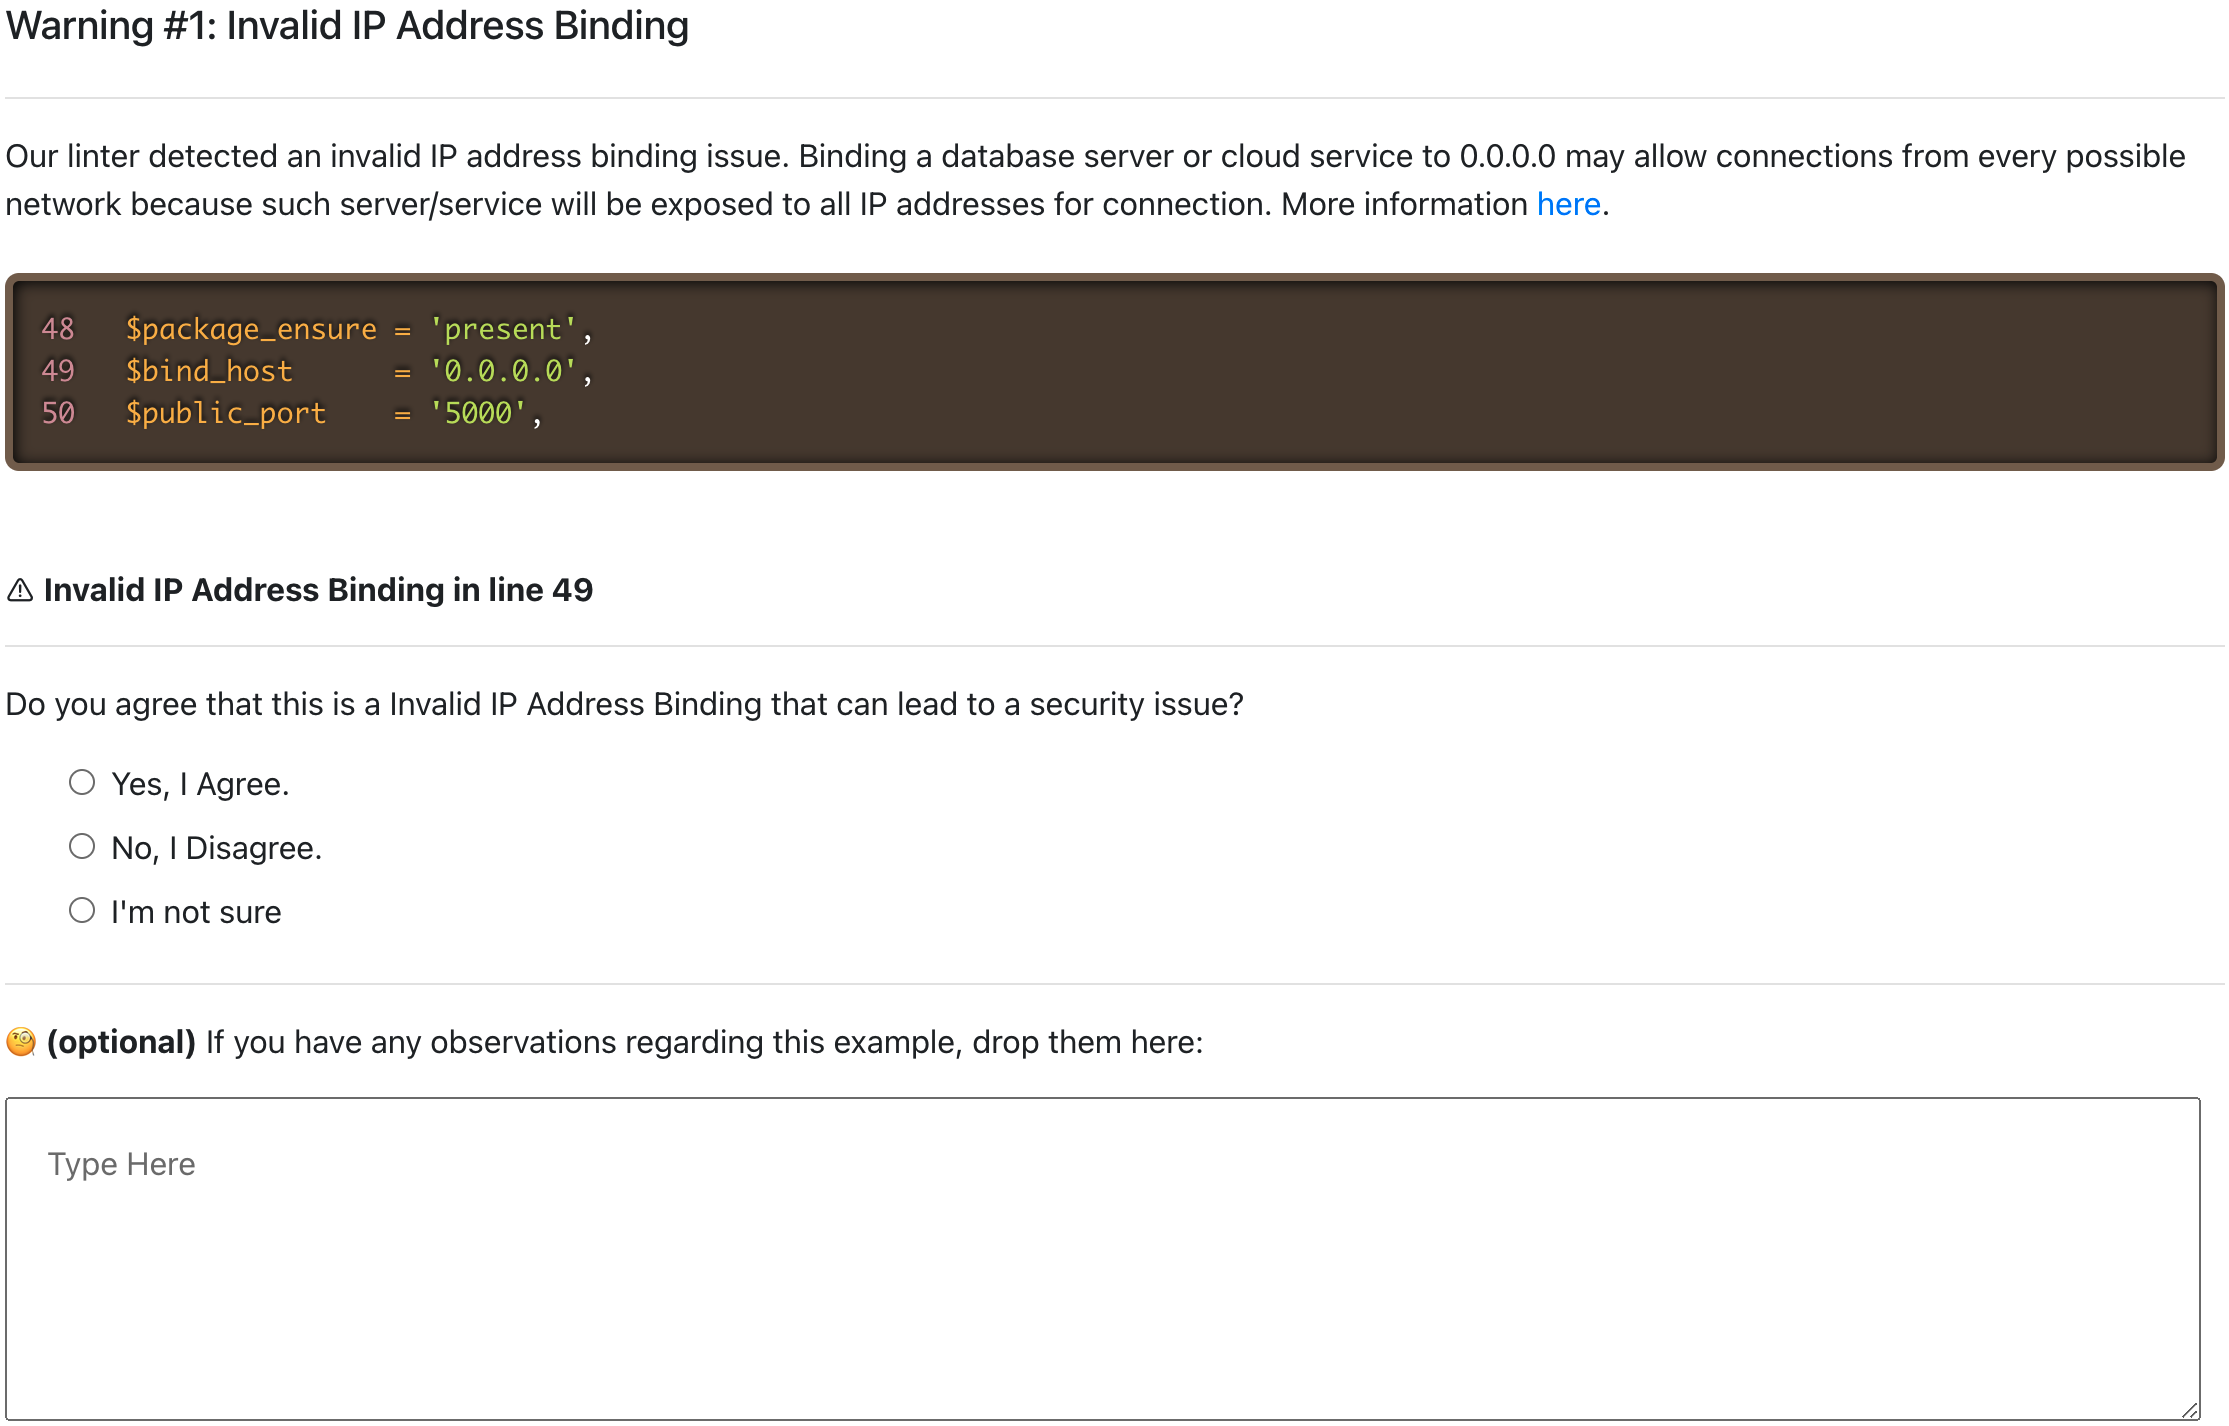
\includegraphics[width=1.05\linewidth]{warning.png}
    \vspace{-3ex}
    \caption{Example of the form presented to the 
    practicioner for warning validation.}\label{fig:warning}
    \vspace{-3ex}
\end{figure}

\textbf{Metrics.} We report the number of true positives (TPs), 
the number of false positives (TPs), the number of ``Unsure'' 
responses and Precision---calculated as described in 
Section~\ref{sec:pre_meth}.

\subsection{Results}
We obtained a total of \noProfessionals{} participants: $74$ in 
the first round of feedback; and $57$ in the second 
round. Due to the lack of responses from participants, we 
were only able to validate $342$ out of the 
$450$ initial number of warnings.
Table~\ref{tab:final_prac} shows the distribution of warnings and 
precision obtained for the final version of \toolname{} (v1.1.0). 
At the end of this study, \toolname{} reported a precision of 
\finalPrecision{}, where $54$ of the warnings  
were False Positives. 

Part of the feedback obtained in this experiment
was documented in Section~\ref{sec:design} and~\ref{sec:rules}.
Table~\ref{tab:infrasecure_prec} shows the evolution 
of the tool's precision with the different iterations of feedback.
In contrast to Table~\ref{tab:prel_analysis_infrasecure}, where 
we report the precision of v0.1.0 for the alerts validated by students;
here, in Table~\ref{tab:infrasecure_prec}, we report the precision of v0.1.0
based on the practitioners' feedback, i.e., leveraging the alerts validated 
by practitioners (instead of students). It is important to 
note that the implementation of v0.1.0 focused on understanding 
variable and attribute assignments and reasoning about the token value  
to reduce the number of incorrect detections. These two improvements affected 
all checkers. The remaining versions of the tool focused on addressing specific 
false positives, extending the ruleset and adding the safe domains feature. 
In the comparison provided in Table~\ref{tab:infrasecure_prec}, we 
observe an increase of precision---from $76\%$
to $83\%$---by conducting different cycles of 
feedback collection.
In addition, feedback was essential to extend 
the ruleset. This study with practitioners led us 
to create $3$ new rules to detect weak passwords;
typosquatting attacks; and malicious dependencies (being 
the last two the root causes of many supply chain attacks~\cite{9402108,duan2020measuring}).

\textit{\textbf{Summary:}} Results show that working side-by-side with the community
will help the authors of the tools develop better linters, 
as proposed before by a Google study~\cite{46576}.
Using this feedback approach, we improved the linter's precision 
and the final ruleset.


\begin{table}[t!]
  \centering
  \small
  \caption{Performance of \toolname{} (v1.1.0). (Validation with Practitioners)}
  \label{tab:final_prac}
  \vspace{-2ex}  
  \begin{tabular}{ p{3.75cm} p{0.5cm} p{0.5cm} p{1cm} p{1cm}} 
    \toprule
    Rule & \#TP & \#FP  & \#Unsure & Precision\\
    \midrule
    Hard-coded secrets & $28$ & $8$ & $3$ & $0.78$ \\
    Use of HTTP without TLS & $32$ & $3$ & $2$ & $0.91$\\
    Suspicious Comments & $16$ & $15$ & $7$ & $0.52$\\
    Use of Weak Crypto. Algo. & $33$ & $3$ & $6$ & $0.92$\\
    Invalid IP Address Binding & $26$ & $8$ & $6$ & $0.77$\\
    Empty Password & $33$ & $3$ & $1$ & $0.92$ \\
    Admin by default & $30$ & $6$ & $6$ & $0.83$\\
    Malicious Dependencies & $25$ & $6$ & $3$ & $0.81$\\
    Weak Password & $32$ & $2$ & $0$ & $0.94$\\
    \midrule
    Total & $255$ & $54$ & $34$ & $0.83$\\
    \bottomrule 
  \end{tabular}
\end{table}

\begin{table}[t!]
  \small
  \centering
  \caption{Precision obtained in different cycles of feedback collection for \toolname{}.}
  \label{tab:infrasecure_prec}
  \vspace{-2ex}  
  \begin{tabular}{p{5cm}p{1.25cm}p{1.25cm}} 
    \toprule
    \textbf{Participants} & \textbf{version} & \textbf{Precision} \\
    \midrule
    Research Team, Owners of OSS Projects, PuppetLabs, Voxpupuli & v0.1.0 &  76\% \\
    Practitioners (cycle 1) & v1.0.0 &  79\%\\
    Practitioners (cycle 2) & v1.1.0 & \finalPrecision \\
    \bottomrule 
  \end{tabular}
  \vspace{-3ex}
\end{table}


\subsection{Discussion \& Limitations}\label{sec:discussion}


This paper reports our approach to improve the ruleset of an IaC security iteratively 
linter in different cycles of feedback collection.
However, the tool can still be improved with more sophisticated 
techniques such as data-flow analysis, which would fulfil the following 
feedback: \textit{In puppet, pre-defining a password as empty does not 
mean it is empty (e.g., \CodeIn{\$ssl\_password    = ''}). Many times 
these variables are changed later. Thus, for each empty password,
\toolname{} verifies if the same variable was changed within the same file.
If it was, then the linter will not raise an issue.}.

In addition, some engineers suggested that usernames 
should be only reported as hard-coded secrets when 
paired with a password/key. For this, we must match the different 
pairs of credentials in a puppet manifest.
To sum up, there are still opportunities 
to improve the precision and recall of \toolname.
We reached out to owners of highly 
active GitHub projects that use Puppet reporting warnings 
detected by \toolname{}. Two owners mentioned that 
since the apps are not in production, they 
did not consider the issues relevant. Even 
after improving the linter to detect the anti-patterns 
correctly, some problems are still not problematic. This happens  
because the linter does not have context regarding 
the software's usage, which will always be a source 
of False Positives. In the future, we will continue to search 
for solutions to make the linter more context-aware
since this is a known problem of linters.

\section{Ethical Standards and Compliance}\label{sec:ethics}

This section discusses compliance with the ACM Policy for Research 
Involving Humans,\footnote{The ACM Policy for Research Involving Humans description is available at \url{https://www.acm.org/publications/policies/research-involving-human-participants-and-subjects} (Accessed \today)} which ensures that the ethical and legal standards 
are met when research has human participants.

\textbf{Informed Consent.} One of the principles is to ensure that 
participants are informed about the fact that they are participating 
in a study. In our study, consent was collected differently for each 
experiment: for the first one, the research team agreed to 
participate in the study; for the OSS maintainers experiment, we used 
the puppet community slack to communicate and discuss the investigation 
with the maintainers; finally, for the practitioners' experiment, we 
asked survey participants if they agreed to participate in our different 
surveys at the beginning of the pre-screening phase. 

\textbf{Data Privacy.} For all experiments, we ensured that the 
participants' private information was protected by not providing 
the participants' personal data (e.g., 
GitHub usernames of the OSS maintainers, prolific participants' 
names, ages, nationalities, etc.) in our replication package. 

\textbf{Spam.} As mentioned in Section~\ref{subsec:maintainers}, 
we carefully organized the issues 
to minimize the amount of messages sent to maintainers~\cite{10.1145/2961111.2962628,10.1145/3379597.3387462}. Security smells of the same kind were all reported in 
a single GitHub issue. In addition, we designed the issues to be 
actionable by providing personalized fix suggestions and 
adding references that document the detected problems.

\textbf{Full Disclosure in Security.} Fully disclosing vulnerabilities on GitHub issues 
allows hackers to exploit unfixed vulnerabilities, creating risks for software users. 
Ideally, vulnerability disclosure should be performed confidentially. Yet, GitHub does not 
provide a feature to report them privately. Therefore, carefully performing full disclosure 
is accepted by OSS maintainers~\cite{fulldisc.2005,askanethcode}. Some OSS projects adopt 
security mailing lists. In those cases, disclosure should be performed through those mailing 
lists. 

\section{Threats to Validity}\label{sec:t2v}

This section presents potential threats to the validity of this study.

\textbf{Internal Validity:} As with any implementation, the scripts that we 
developed to run the tools and collect the metrics 
reported in the paper are potentially not bug-free. However, the scripts and 
outputs are open-source for other researchers and
potential users to check the validity of the results. 

\textbf{Construct Validity:} A potential threat is the manual analysis
of the warnings raised by \slic{} in the Puppet scripts, which can potentially be 
mislabeled. We tried to mitigate this by running a kappa analysis between the two co-authors. 
For the experiments with the OSS maintainers, 
we inferred the validations of the alerts from their comments. Although both co-authors inferred the validations, and a kappa analysis was performed, we risk our inference being incorrect. It is also important to mention 
that even though we made an effort to collect feedback from experienced humans,
their judgement can also not be $100\%$ accurate, which can introduce error  
in the precision values reported.

\textbf{External Validity:} A potential threat to external validity 
is related to the fact that the set of Puppet scripts we have considered 
in this study may not accurately represent the whole set of 
vulnerabilities that can happen during development. We attempt to reduce
the selection bias by gathering a large collection of real, openly 
available (hence, reproducible) Puppet scripts. Another potential threat 
is that we could have missed the latest updates to \slic{}. To
mitigate this risk, we contacted the authors of \slic{} to confirm that 
the version available is true to the most recent one. 
%
\section{Related Work}\label{sec:rw}
%
As IaC has become popular and prevalent, researchers 
have dedicated efforts to improve its quality. Jiang \etal{} conducted
an empirical study on Puppet scripts to gain a deep understanding of the 
characteristics of such scripts and how they evolve over 
time~\cite{7180066}. Bent \etal{} investigated the quality and
maintainability aspects of Puppet scripts~\cite{van2018good}. 
Furthermore, Rahman \etal{} proposed prediction models (based on text
mining) to classify defective IaC scripts~\cite{rahman2018characterizing}. 
Palma \etal{} created a catalog of software metrics for IaC scripts ~\cite{dalla2020towards}. 
In addition, recent work has been developed to detect malicious
packages published on registry maintainers such as npm and ruby
gems~\cite{duan2020measuring}. Building and introducing linters 
earlier in the software development life-cycle shift security 
left and decreases the probability of shipping malicious packages.

There are several linters available for security but only the subject of
this paper, \slic{}, focuses in IaC scripts for Puppet~\cite{8812041}. 
The authors started by demonstrating the linter in the context of Puppet
scripts, and later, the authors reproduced the same study for Chef and 
Ansible and created new tools for those technologies~\cite{10.1145/3408897}. 
A major issues with linters is their lack of precision~\cite{park2016battles,muske2016survey,gauthier2018scalable,landman2017challenges,christakis2016developers,vassallo2020developers}: 
low precision entails low reliability for developers. Previous research 
has shown the impact of this issue on the developers' workflow and stressed 
it is essential to create precise tools; otherwise, the developers 
will not use them~\cite{6606613,7781843,10.1145/1646353.1646374,8622456,8530713,46576}.
As mentioned before, this study aims to gain a better 
understanding of the current capabilities of the only IaC security linter for 
Puppet and shed some light on how to move forward.

%
\section{Conclusions \& Future Work}\label{sec:conclusion}
%
In this study, we observed through a comprehensive study that 
security linters for IaC scripts still need to be improved to 
be adopted by the industry. This paper leverages community expertise 
to address the challenge of improving the precision of such linting 
tools. We focused on precision as it is critically important 
in this domain---false security warnings can be very disruptive. 
More precisely, we interviewed professional developers
of Puppet scripts to collect their feedback on the root causes of
imprecision of the state-of-the-art security linter for Puppet. From
that feedback, we developed a linter adjusting \noRulesSlic\ rules
of an existing linter ruleset and adding \newRules\ new rules. We
conducted a new study with \noProfessionals\ professional developers,
showing an increase in precision from \botPrecision\ to \finalPrecision.
Following the findings of a Google study~\cite{46576}, we show that 
authors of linters can improve their own tools if they focus 
on the users' feedback.
The takeaway messages of this paper are that (i) it is feasible to
tune security linters to produce acceptable precision; and, that 
(ii) involving practitioners in
discussions is an effective way to guide the improvement of those
linters. 

The observations that we made throughout this work pave the
way for the following future work: extend \toolname\ to detect other
security vulnerabilities, integrate the tool with methods for
automated patching, and port \toolname\ to other configuration
management tools.
